\documentclass[journal]{IEEEtran}

\usepackage{cite}
\usepackage{amsmath,amssymb,amsfonts,amsthm}
\theoremstyle{definition}
\newtheorem{criterion}{Criterion}
\usepackage{graphicx}
\graphicspath{{figures/}}
\usepackage{textcomp,xcolor,booktabs,array,url,enumitem,multirow}
\setlist{topsep=2pt,itemsep=1pt,parsep=0pt,leftmargin=*}
\usepackage{tikz}
\usetikzlibrary{positioning,arrows.meta,fit,backgrounds,automata,shapes.geometric}
\usepackage{pgfplots}
\pgfplotsset{compat=1.18,table/col sep=comma}
\usepgfplotslibrary{groupplots}
\emergencystretch=1em
\setlength{\textfloatsep}{6pt plus 2pt minus 2pt}
\setlength{\floatsep}{4pt plus 2pt minus 2pt}
\setlength{\dblfloatsep}{6pt plus 2pt minus 2pt}
\setlength{\dbltextfloatsep}{6pt plus 2pt minus 2pt}
\setlength{\intextsep}{4pt plus 2pt minus 2pt}
\setlength{\abovecaptionskip}{3pt}
\setlength{\belowcaptionskip}{0pt}

\begin{document}

\title{DIB: Managing Local MUD Policy Lifecycles with Shared IoT Traffic Evidence}
\author{Anonymous Authors}
\maketitle

\begin{abstract}
Shared IoT traffic observations can support Manufacturer Usage Description (MUD) policy drafting across independent administrative domains, but provide evidence, not local authority. Device Intent Blueprint (DIB) separates shared evidence from per-site authorization through explicit approval, dispute, revocation, and restoration semantics. Only local operators authorize export; disputes invalidate authorization, and restoration requires renewed approval while preserving local revocations. A finite TLA+ model checks these properties across 3,837,084 reachable states; mutation controls expose restoration and site-confinement failures, and registry regression testing identified and corrected a revocation-handling mismatch. An OpenWrt/osMUD testbed validates policy application on a reachable gateway. A single-host, ten-site distributed deployment reconciles disconnected sites in 0.51~s; an extended finite model checks safety only among reachable, reconciled sites. A matched cold-start comparison across three deployments and six device types reduces candidate counts by 92.3--96.4\% relative to pooled observations, cutting review cost from 4.3--28.3 to 1.03--2.89 inspected candidates per confirmed endpoint while lowering recall. Quorum drives most of the reduction; additional filters have receiver-dependent costs. A separate reference-profile evaluation retains 63.2\% of observable macro behavior with 7.9\% complete-profile recall. DIB manages partial policy proposals under authenticated-consortium assumptions; it neither establishes benignity nor guarantees immediate withdrawal at unreachable gateways.
\end{abstract}

\begin{IEEEkeywords}
IoT security, Manufacturer Usage Description, distributed network management, access policy management, policy lifecycle.
\end{IEEEkeywords}

\section{Introduction}
\label{sec:introduction}
Manufacturer Usage Description (MUD)~\cite{rfc8520} lets an Internet-of-Things (IoT) device advertise its intended communications, which a MUD manager translates into access-control rules. Manufacturer profiles may be unavailable or become stale as firmware and cloud services change~\cite{hernandezramos2021mudreview,allowlistvariability}; traffic observations can help draft or update them.

Sharing observations across administrative domains can seed proposals before sufficient local traffic is collected. An endpoint needed in one network may be unnecessary elsewhere, and compromised devices may contact attacker-controlled destinations~\cite{allowlistvariability,mirai}. Remote observations therefore supply evidence, not authority: cross-network agreement can prioritize review, while only the receiving site's operator can authorize activation.

Consider a camera without a manufacturer profile: two peer networks report a service, which the local administrator approves. A peer later disputes it. The management system must invalidate approval, propagate withdrawal to the gateway, and resolve the dispute without reusing old permissions or overriding local revocations. An approval prompt alone specifies neither this lifecycle nor reconciliation after disconnection.

We present \emph{Device Intent Blueprint (DIB)}, a policy-management framework for independently administered networks, or \emph{sites}. A shared \emph{registry} separates evidence from per-site authorization records. An \emph{endpoint fact} identifies a communication by device type, direction, protocol, peer, and port. Eligible facts enter review as \textsc{MonitorOnly}, producing no MUD entry or firewall rule. A local approval, or \emph{commit}, makes the record \textsc{Active}, authorizing MUD export. Gateway fetch and application are separate: registry withdrawal does not immediately remove a rule at an unreachable gateway.

DIB tracks approval validity and revocation origin so restoration after shared withdrawal requires fresh approval without erasing local vetoes. This lifecycle, rather than traffic classification, is the management contribution; candidate filtering controls proposal volume without establishing benignity.

The paper makes three contributions:
\begin{itemize}
\item \textbf{Lifecycle semantics.} We separate shared evidence from local authority and define approval, dispute, revocation, restoration, and export transitions. A finite TLA+ model checks authorization safety and preservation of local vetoes over 3,837,084 reachable states.
\item \textbf{Execution and reconciliation.} A registry and OpenWrt/osMUD testbed connect lifecycle decisions to MUD export and firewall updates. A ten-site distributed deployment tests reconciliation after missed dispute/restore events; an extended finite model checks safety among reachable, reconciled sites.
\item \textbf{Proposal-volume trade-offs.} UNSW-IoTraffic~\cite{sivanathan2019classifying}, Mon(IoT)r~\cite{moniotr}, and YourThings~\cite{alrawi2019yourthings} experiments quantify candidate reduction, coverage loss, and cold-start transfer. Matched ablations isolate quorum and filter effects; adversarial tests distinguish conditional rejection from empirical mitigation.
\end{itemize}

\section{Related Work}
\label{sec:related-work}
RFC~8520 leaves MUD profile authoring and management to administrators~\cite{rfc8520}. Prior work extracts or enforces profiles from local traffic within one administrative domain~\cite{clearasmud,hamzatdsc,mudflow,CornoMannella2023GatewayMUD,osmud,mudscope}, rather than governing shared observations across domains.

Threat-intelligence sharing (MISP, STIX), contributor reputation~\cite{wagner2016misp,stix21,eigentrust,trustsurvey}, and collaborative IoT learning (CoLearn, D\"IoT, IoT Inspector)~\cite{colearn,ndiot2019,iotinspector,vasilomanolakis2015collaborative} provide related mechanisms for aggregating evidence, traffic models, or anomaly reports. Evidence quality alone does not authorize network reachability.

Cross-domain policy frameworks address distributed authoring, provenance, or consistency~\cite{pbnm,rfc9315,matheu2019mudtesting,blockchainmud,fidem,liuzerotrust2024,sun2025sanitizable,polaris,alshaer2004firewall,chowdhary2022intent,pipeconf2022,vergutz2023data}. DIB focuses on how shared disputes and restoration interact with independent local decisions. No published system combines MUD policy objects, evidence contributed across administrative domains, and a per-site authorization record with dispute-driven withdrawal and restoration. MUD work operates inside one domain~\cite{clearasmud,hamzatdsc,mudflow,CornoMannella2023GatewayMUD,osmud,mudscope}; cross-domain access-control frameworks operate on identity and policy objects carrying no notion of contributed traffic evidence~\cite{polaris,liuzerotrust2024,sun2025sanitizable}; evidence-sharing platforms distribute indicators without a local authorization record to invalidate~\cite{wagner2016misp,stix21,colearn,ndiot2019}; and blockchain-backed MUD distribution~\cite{blockchainmud} makes profiles tamper-evident without separating shared evidence from site-local authority. The available reference points are therefore the two ends of the design space DIB sits between: pooled union, which stages every shared observation, and reputation-weighted voting, which weights contributors but still yields one shared verdict. We evaluate against both (Sec.~\ref{sec:impl}). Table~\ref{tab:comparison} accordingly compares defined workflow semantics: the alternatives are the restoration rules a system can implement, not deficiencies of any particular prior system. DIB contributes their composition for shared MUD proposals, finite-state verification, and executable withdrawal and re-approval.

\begin{table}[t]
\centering
\caption{Defined workflow alternatives for one fact, initially approved at site $s$. The sequence is local revoke at $s$, peer dispute, then global restore.}
\label{tab:comparison}
\scriptsize
\begin{tabular}{@{}p{2.1cm}p{2.3cm}p{2.65cm}@{}}
\toprule
Workflow & Global-restore rule & Result at $s$ \\
\midrule
Approval + persistent approval bit & Reuse old approval & Permission can return without fresh approval \\
Approval + review reset & Reset all revoked records to review & No permission, but local veto is erased \\
Provenance-aware review (DIB) & Reset only dispute-derived records & Local revocation survives; no permission \\
\bottomrule
\end{tabular}
\end{table}

\section{Threat Model and Goals}
\label{sec:threat}

We consider a closed consortium of sites controlling their own gateways. Remote reports are distinct from local authorization.

\subsection{Setting and Trust Boundary}
\label{subsec:trust}
The deployment is assumed to authenticate consortium membership out-of-band (e.g., mutual TLS with enterprise PKI), reject unauthenticated contributions, encrypt and authenticate registry communication, and enforce identities and roles. Device-taxonomy alignment is assumed complete before ingestion. Admission additionally assumes malicious contributors control at most fraction $f_s$ of the eligible reporting population for a device type (Sec.~\ref{sec:scoring}); identity-inflation tests deliberately exceed this bound.

We evaluate three distinct adversarial behaviors: (i)~\textbf{A1 (Poisoned Observations),} where an honest site captures and reports real malicious flows from an already compromised device; (ii)~\textbf{A2 (Fabricated Evidence),} where contributors report fabricated traffic that did not occur (bounded by breadth share $f_s$, or unbounded in Sybil stress tests); and (iii)~\textbf{A3 (Low-and-Slow Behavioral Drift),} where attacker activity is distributed across sites to mimic a legitimate rollout.

Local operators are sovereign within their domain: misuse of a local commit or revocation is an insider threat, not a cross-site authorization failure. Attackers may pollute review queues or disrupt availability through baseless disputes, but disputes are restrictive and cannot create \textsc{Active} authorization. A3 exposes an observational limit: identical traffic patterns yield identical scores regardless of benignity or intent~\cite{mirai,allowlistvariability}. Without a local commit, admitted patterns remain unprivileged \textsc{MonitorOnly} candidates. Authorization tokens belong to the receiving site's local state and cannot be created by remote contributors.

\textbf{Consortium authority.} A participating site can raise a dispute; the first dispute suspends export and a second distinct site confirms revocation. Global restoration is a privileged consortium operation whose authorization must be supplied by the deployment, and local approval, revoke, and restore must be bound to the receiving site's operator: local control means exclusive creation of permissions, while consortium members accept shared emergency withdrawal. This deliberately favors restriction over availability, as a malicious member can interrupt service.

\textbf{Scope of the safety properties.} I1--I3 (Sec.~\ref{subsec:lifecycle}) concern lifecycle transitions under authenticated identities. The prototype and finite model expose transitions to a trusted harness; correct caller authentication and role enforcement are deployment assumptions, not implemented or verified mechanisms.

\subsection{Design Goals}
We formulate five core design goals:
\begin{itemize}
\item \textbf{G1 (Local Authorization Sovereignty):} Export only locally approved endpoint facts representable as valid MUD access-control entries (ACEs).
\item \textbf{G2 (Zero-Profile Bootstrapping):} Propose review candidates for newly observed devices even when manufacturer profiles are absent.
\item \textbf{G3 (Candidate-Volume Reduction):} Reduce the number of proposals presented for review relative to pooling all observations.
\item \textbf{G4 (Non-Destructive Rescoring):} Allow evolving evidence to update candidate scores without silently altering existing local approvals.
\item \textbf{G5 (Adversarial Rejection):} Reject facts supported only by malicious contributors when their population share and the score parameters satisfy the bound in Section~\ref{sec:scoring}.
\end{itemize}
G1 and G4 protect authorization; G2, G3, and G5 concern candidate quality. Gateways determine effective enforcement.

\section{Device Intent Blueprint}
\label{sec:design}
DIB separates candidate admission, site-local export authorization, and gateway application.

\subsection{Records and Operational Flow}
\label{subsec:endpoint-facts}
For device type $d$, an endpoint fact is $f=(d,e)$, where $e=(\text{direction},\text{protocol},\text{peer},\text{port})$. The peer is an FQDN or remote IP address; normalization prefers an observed FQDN when available. Scoring uses outbound tuples since the evaluated traffic predominantly concerns device-initiated communications; the exporter can also generate return-flow ACEs.

The registry keeps two kinds of record. \emph{Shared evidence records} store observations, reporters, timestamps, and attestations as audit provenance: \textsc{contribute} records traffic idempotently, \textsc{attest} records a site's explicit stance on an admitted fact, and reporter counts give audit tiers (Local, Corroborated, Consortium-attested) that help review but grant no permission. \emph{Site-local authority records} store each receiving site's decision, approval validity, and revision history independently of the evidence.

\textbf{Following the camera proposal.} In Sec.~\ref{sec:introduction}'s example, eligibility, reporter count, persistence, and dispute checks (Sec.~\ref{sec:scoring}) produce a \textsc{MonitorOnly} proposal, not a packet-monitoring rule. Local approval creates fresh authorization in \textsc{Active}; the serializer emits a MUD ACE for the gateway to fetch and apply.

A dispute invalidates authorization at all sites; gateways must apply the regenerated policy to withdraw installed permissions. A second independent dispute confirms revocation. Restoration returns applicable records to review without erasing local revocations (Table~\ref{tab:transitions}); Fig.~\ref{fig:admission-flow} shows the forward path.

\begin{figure}[t]
\centering
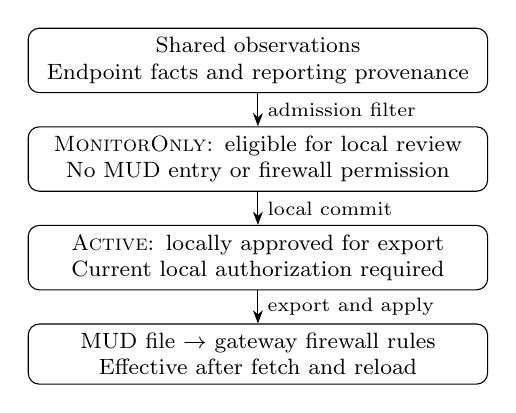
\begin{tikzpicture}[>=Stealth,every node/.style={font=\footnotesize},
stg/.style={draw,rounded corners,align=center,text width=5.6cm,minimum height=0.65cm},
node distance=0.42cm]
\node[stg] (evidence) {Shared observations\\Endpoint facts and reporting provenance};
\node[stg,below=of evidence] (review) {\textsc{MonitorOnly}: eligible for local review\\No MUD entry or firewall permission};
\node[stg,below=of review] (active) {\textsc{Active}: locally approved for export\\Current local authorization required};
\node[stg,below=of active] (gateway) {MUD file $\rightarrow$ gateway firewall rules\\Effective after fetch and reload};
\draw[->] (evidence)--node[right,font=\scriptsize]{admission filter}(review);
\draw[->] (review)--node[right,font=\scriptsize]{local commit}(active);
\draw[->] (active)--node[right,font=\scriptsize]{export and apply}(gateway);
\end{tikzpicture}
\caption{Separate evidence, authorization, and enforcement steps. Admission creates proposals; local commit authorizes export; gateway application changes connectivity. Withdrawal invalidates authorization; restoration requires renewed approval.}
\label{fig:admission-flow}
\end{figure}

\subsection{Site-Local Authority Lifecycle}
\label{subsec:lifecycle}
At each site $s$, an endpoint fact $f$ resides in one of five authorization states:
\[
S=\{\text{Absent},\text{MonitorOnly},\text{Active},\text{Disputed},\text{Revoked}\}.
\]
These states track administrative authorization, distinct from gateway enforcement. \textsc{Active} indicates that site $s$'s operator has authorized fact $f$ for policy export. Each approval creates a fresh local authorization instance. The Boolean $\texttt{grantValid}[s][f]$ records whether that instance remains valid; here, ``token'' denotes authorization state, not a bearer credential. A fact is exportable if and only if:
\begin{equation}
\begin{aligned}
\mathrm{Exportable}(s,f) \iff{}&\ \mathrm{state}(s,f)=\textsc{Active}\\[-2pt]
&\land\ \mathrm{grantValid}(s,f).
\end{aligned}
\label{eq:exportable}
\end{equation}

Let $\Sigma$ be the lifecycle events, including queries, commits, disputes, and restorations. We write $\delta: S\times\Sigma\rightarrow S$ for the state projection of the record transition; guards also depend on authorization validity, dispute status, and revocation origin (Table~\ref{tab:transitions}). Absent means not staged; Disputed means suspended; Revoked retains whether withdrawal was local or dispute-derived.

\begin{table*}[t]
\centering
\caption{Lifecycle transitions. A second dispute must come from a site distinct from the opener. Undefined transitions leave the record unchanged or are rejected.}
\label{tab:transitions}
\scriptsize
\begin{tabular}{@{}llllll@{}}
\toprule
Current state & Event & Precondition & Next state & Token valid? & Exportable? \\
\midrule
Absent & query/stage & admitted; no open dispute & \textsc{MonitorOnly} & no & no \\
\textsc{MonitorOnly} & local commit & local operator; no dispute & Active & yes, new & yes \\
\textsc{MonitorOnly}/Active & first dispute & valid dispute & Disputed & no & no \\
Disputed & second dispute & distinct reporting site & Revoked (Dispute) & no & no \\
Disputed/Revoked (Dispute) & global restore & authorized restore & \textsc{MonitorOnly} & no & no \\
Active/\textsc{MonitorOnly} & local revoke & local operator & Revoked (Local) & no & no \\
Revoked (Local) & local restore & no open dispute & \textsc{MonitorOnly} & no & no \\
Revoked (Local) & global restore & --- & Revoked (Local) & no & no \\
Absent & dispute & --- & Absent & no & no \\
\bottomrule
\end{tabular}
\end{table*}

Local revoke is defined only from Active or \textsc{MonitorOnly}, not from Disputed or Revoked (Dispute). Thus an operator cannot add an independent veto during suspension or after dispute-confirmed revocation. This matters because global restore returns dispute-derived records to review but must preserve local vetoes (I3). Local revoke becomes available again in \textsc{MonitorOnly}; local restore cannot release Revoked (Dispute). Extending veto recording to these states and re-verifying the lifecycle remain future work.

\textbf{Core Invariants (I1--I3).} Under the stated identity assumptions, the lifecycle requires:
\begin{itemize}
\item \textbf{(I1) Fresh Local Authorization:} Only an explicit \textsc{operator-commit} by site $s$'s operator can transition a fact to \textsc{Active} and generate a valid authorization token. No sequence $\sigma$ of non-commit events (i.e., $\sigma\in\Sigma_{\text{non-commit}}^*$, any sequence drawn from events other than operator-commit) can enter \textsc{Active}, where $\hat\delta$ extends $\delta$ to sequences:
\[
\forall s,f:\quad \hat{\delta}(\text{Absent}, \sigma) \neq \text{Active}, \quad \forall \sigma \in \Sigma_{\text{non-commit}}^*.
\]
\item \textbf{(I2) Site Confinement:} Local actions (\textsc{operator-commit}, \textsc{local-revoke}, \textsc{local-restore}) at site $s$ have no side effects on any peer site $s' \neq s$.
\item \textbf{(I3) Conservative Reversal:} A dispute immediately clears export eligibility and invalidates authorization tokens across all sites. Restoration conservatively returns records to \textsc{MonitorOnly} without regenerating tokens, requiring fresh local re-authorization. Global restoration never overrides an independent local revocation.
\end{itemize}

\textbf{Registry safety and gateway application.} Let $\mathrm{Exported}(s,f,t)$ denote an export event at time $t$. We call $\mathrm{CurrentLocalAuthorization}(s,f,t)$ true when the record is \textsc{Active}, its approval was created by a local commit, and that approval has not been invalidated. The registry must satisfy
\begin{equation}
\begin{split}
\mathrm{Exported}(s,f,t)\ \Rightarrow\\
\mathrm{CurrentLocalAuthorization}(s,f,t).
\end{split}
\label{eq:export-authority}
\end{equation}
The finite model checks this property together with I1--I3.

The testbed checks rule creation and removal after gateway policy application, not instantaneous synchronization. An unreachable gateway may retain an older rule after registry invalidation. Conversely, an admission error can add an unsuitable review candidate without authorizing any rule.

\subsection{Candidate Admission}
\label{sec:scoring}
Admission controls proposal volume, not authorization. A fact reaches review only if it passes endpoint-class eligibility, reporter quorum, score, and dispute checks (Eq.~\ref{eq:admitauto}); Table~\ref{tab:symbols} gives the operating values.

\begin{table}[t]
\centering
\caption{Admission notation and defaults. Sec.~\ref{sec:sensitivity-results} varies $m$, $\theta$, and $\alpha$; Sec.~\ref{sec:security-results} varies the realized $f_s$.}
\label{tab:symbols}
\scriptsize
\begin{tabular}{@{}p{1.3cm}p{5.00cm}p{0.75cm}@{}}
\toprule
Symbol & Meaning & Value \\
\midrule
$d$, $e$ & device type; endpoint (direction, protocol, peer, port) & --- \\
$A(d,e)$ & endpoint-class eligibility (the class gate) & --- \\
$ES_d$ & sites with at least one observation of device type $d$ & --- \\
$S_{d,e}$ & subset of $ES_d$ that reports endpoint $(d,e)$ & --- \\
$C_s$ & cross-site breadth, $|S_{d,e}|/|ES_d|$ & --- \\
$C_t$ & temporal-persistence confidence (Eq.~\ref{eq:ct}) & --- \\
$D_{d,e}$, $D_d$ & UTC dates observing $(d,e)$; dates observing any endpoint of $d$ & --- \\
$n_{d,e}$, $n_d$ & pooled observation counts for $(d,e)$; for all of $d$ & --- \\
$score(d,e)$ & admission score, $\alpha C_s+\beta C_t$ (Eq.~\ref{eq:score}) & --- \\
$C_s^{trust}$ & trust-weighted breadth (Eq.~\ref{eq:trustweight}) & --- \\
$w_i$, $b_i$, $b_{ref}$ & site $i$'s trust weight; distinct fact breadth; reference breadth & --- \\
$m$ & minimum reporting sites (quorum) & 2 \\
$\theta$ & admission threshold & 0.65 \\
$\alpha,\beta$ & breadth / temporal weight, $\alpha+\beta=1$ & 0.6, 0.4 \\
$f_s$ & assumed adversarial breadth share & 0.30 \\
\bottomrule
\end{tabular}
\end{table}

\textbf{Eligibility.} After address filtering, $A(d,e)=1$ for DNS, NTP, update, or vendor-cloud endpoints: DNS is \texttt{dns} or port 53, NTP is \texttt{ntp} or port 123, update names contain \texttt{update}/\texttt{upgrade}/\texttt{firmware}/\texttt{ota}/\texttt{fw.}/\texttt{-fw}/\texttt{swupdate}, and vendor-cloud is any remaining FQDN; private, reserved, and link-local IP literals fail. We call this the \emph{class gate}: a resolvability/control-plane filter, not an intent classifier, so a resolved attacker domain still clears it (Sec.~\ref{sec:security-results}).

Breadth is the fraction of sites observing device type $d$ that report this endpoint: $C_s=|S_{d,e}|/|ES_d|$, where $ES_d$ contains every site with at least one observation of $d$ and $S_{d,e}$ those reporting $(d,e)$ specifically (a site need not report this endpoint to enter the denominator) --- a site-population definition distinct from the endpoint-class gate $A(d,e)$.
Let $D_{d,e}$ be the union of UTC calendar dates of observations of $(d,e)$ across sites, $D_d$ the corresponding union for all observations of $d$, and $n_{d,e}$, $n_d$ their pooled observation counts. Temporal confidence, combining day coverage and frequency, is
\begin{equation}
C_t=0.7\frac{|D_{d,e}|}{|D_d|}+0.3\frac{n_{d,e}}{n_d}\in[0,1].
\label{eq:ct}
\end{equation}

\textbf{Admission score.} Nonnegative weights $\alpha$ and $\beta$ determine the contributions of breadth and persistence, respectively. The score is
\begin{equation}
score(d,e)=\alpha C_s(d,e)+\beta C_t(d,e),
\qquad \alpha+\beta=1 .
\label{eq:score}
\end{equation}

\textbf{Combined rule.} Let $\theta$ be the minimum score and $openDispute(d,e)$ indicate an unresolved dispute. We require at least two distinct reporting sites ($m=2$, the quorum); a larger quorum requires more reports and can delay admission, since authenticated identities alone do not establish independent behavior. Automatic admission to review is
\begin{equation}
\begin{aligned}
\mathrm{admit}_{auto}(d,e)
={}&(A(d,e)=1)\wedge(|S_{d,e}|\ge m)\\
 &{}\wedge(score(d,e)\ge\theta)\\
 &{}\wedge\neg openDispute(d,e).
\end{aligned}
\label{eq:admitauto}
\end{equation}
Registry queries block disputed/revoked facts; \textsc{operator-commit} remains necessary for Active.

We select weights from an external adversarial-breadth bound and threshold, then measure utility: raw-breadth parameters are $(\alpha,\beta)=(0.6,0.4)$, $\theta=0.65$, and $m=2$. Sec.~\ref{sec:sensitivity-results} reports the empirical cost.

\textbf{Parameter selection.} The weights are not tuned on the corpus. We fix them from the external breadth bound, so admission arithmetic decides $\alpha$ before any dataset is seen.

\begin{criterion}[Admission design constraint]
\label{crit:poison-bound}
If malicious contributors hold at most breadth share $f_s$ of the eligible population and an endpoint fact is reported only by them, then $C_s\le f_s$ and $C_t\le1$, so
\begin{equation}
score(d,e)\le\alpha f_s+\beta
=1-\alpha(1-f_s).
\label{eq:poisonbound}
\end{equation}
Requiring this upper bound to fall strictly below $\theta$ constrains the parameters to $\alpha>(1-\theta)/(1-f_s)$, equivalently $f_s<1-(1-\theta)/\alpha$.
\end{criterion}

The constraint is what selects the operating point. At $\theta=0.65$ and $f_s=0.30$ it admits no $\alpha\le0.5$: a design weighting persistence at least as heavily as breadth could be carried past $\theta$ by fabrication volume alone. We take $\alpha=0.6$, which bounds an adversary-only score at 0.58 and tolerates breadth shares below about 0.42; Sec.~\ref{sec:sensitivity-results} prices this choice against the corpus optimum. The constraint is an arithmetic property of Eq.~\ref{eq:score}, not a security theorem: it inherits whatever bound the deployment governs $f_s$ by, applies to raw breadth $C_s$ only, and says nothing about contributors who accumulate genuine breadth. The bounded-A2 sweep and the port-masquerading counterfactual therefore use raw $C_s$; Sec.~\ref{sec:sybil-results} evaluates the trust-weighted and clustered variants empirically, and the temporal split within $\beta$ is heuristic.

\textbf{Sybil-aware variants.} Trust weighting replaces raw breadth with
\begin{equation}
C_s^{trust}=\frac{\sum_{i\in S_{d,e}}w_i}{\sum_{i\in ES_d}w_i},
\qquad w_i=\min(1,b_i/b_{ref}),
\label{eq:trustweight}
\end{equation}
where $b_i=|\{(d,e):i\text{ contributed }(d,e)\}|$ is site $i$'s distinct fact breadth across device types and $b_{ref}$ is the median of these breadths in a frozen clean snapshot built before injection. $b_i$ is recomputed on the population currently being scored, so every site---including a newly appearing identity---is weighted by its own present breadth, and padding raises $b_i$ directly; only $b_{ref}$ is frozen. This differs from the Reputation-Weighted Voting (RWV) reference point (Sec.~\ref{sec:impl}), which instead fixes weights once on the pre-attack population, giving an absent identity a flat probation weight regardless of later behavior.

Clustering groups sites with similar endpoint sets: for each device type, sites are graph vertices, an edge joins sets with Jaccard similarity (intersection over union) at least 0.8, and each connected component counts as one source. Writing $c(i)$ for site $i$'s component, clustered breadth is $|\{c(i):i\in S_{d,e}\}|/|\{c(i):i\in ES_d\}|$.

The registry and independent-deployment experiments use raw breadth. The UNSW retention funnel uses trust weighting; the identity-inflation experiment compares raw, weighted, and clustered variants. Weighting and clustering do not inherit Criterion~\ref{crit:poison-bound}'s guarantee and depend on a clean reference or meaningful endpoint diversity.

\textbf{Limitations.} Days are unioned while counts are pooled, so busy sites affect frequency. Fleet changes can also rescore unrelated facts (Sec.~\ref{sec:drift-results}).

\section{Implementation and Method}
\label{sec:impl}
The conceptual baseline is pooled union plus local approval, without the lifecycle semantics of Sec.~\ref{sec:related-work}.

The single-node Python registry (FastAPI, SQLAlchemy~2, SQLite) separates evidence/admission from local authority, flags, and history. Transactions atomically fan out dispute/restore for one fact; conflicting writes retry up to ten times. The API recomputes admission from stored observations and exports currently authorized facts as MUD; gateway fetch/reload remain separate. Distribution requires coordination of these transitions (Sec.~\ref{sec:scalability-results}).

\textbf{Datasets.} We use UNSW-IoTraffic~\cite{sivanathan2019classifying}, Mon(IoT)r~\cite{moniotr}, and YourThings~\cite{alrawi2019yourthings}; Sec.~\ref{sec:loo-results} uses the latter as a third independent deployment. UNSW supplies 27 device types and 28 traffic-derived reference profiles; its one physical capture is shuffled round-robin into ten seeded pseudo-sites (seed 42 unless stated). Collapsing Mon(IoT)r VPN variants yields independent US and UK captures, with 3,484,201 of 4,166,133 records surviving address filtering. Adapters require the five endpoint fields: UNSW uses same-site Host/SNI evidence for 24-hour IP-to-name correlation, Mon(IoT)r uses cumulative DNS, and we retain device-initiated transport flows with a port and global peer or public name. The serializer emits RFC~8520's resolved-name TCP/UDP subset, not RFC~9761 TLS/DTLS extensions~\cite{rfc9761}; 0.9\% of reference ACEs (0.6\% macro) are unrepresentable. Adapters and manifests are in the artifact.

\textbf{Reference points.} \emph{Local-only} uses receiver facts; \emph{pooled union} stages every fact. Its approval variant leaves Active records unchanged when evidence changes; a simple revoke permits withdrawal but specifies neither dispute fan-out nor restoration. DIB defines these semantics; this lifecycle comparison is not separately benchmarked. The admission ablation starts with \emph{quorum-only} (two reporters), then adds scoring and class eligibility. \emph{Frequency filtering} requires $n_{d,e}\ge2$; the \emph{50\% registry}, $|S_{d,e}|/|ES_d|\ge.5$; and \emph{RWV}, weighted support $>0.65$. RWV freezes pre-attack weights and assigns new identities 0.1, scaling with raw Sybil count unlike DIB's dynamic weighting.

\textbf{Ground truth and randomization.} Predictions match device, direction, normalized protocol, peer, and port; port 0, unknown protocol, and CIDR ranges are handled as wildcards or membership. Micro metrics pool true/false positives/negatives; macro metrics average over the 28 UNSW reference profiles. Independent-deployment precision/recall/F1 measure agreement with the receiving site's observed traffic, not a manufacturer policy. Aggregates use seeds 0--19; A1, Sybil, and drift use seed 42, and cross-lab, OpenWrt, and concurrency use seed 0.

\textbf{Enforcement testbed.} A privileged Docker container with the OpenWrt 23.05.5 root filesystem runs unmodified osMUD commit \texttt{852918e}, restarted per policy change to materialize MUD ACLs as nftables rules. Each transition records ACEs, effective rules, registry/osMUD state, and a live TCP probe. Unsigned experimental exports require disabling signature validation; production requires signed MUD and PKI.

\textbf{Captured and synthetic events.} A1 replays 165 captured malicious observations forming 59 facts to $k$ pseudo-sites. Other tests inject fabrications, resolved-name and port masquerading, Sybil identities (200--3,200; 20--400 days), and rollouts, with endpoint sets diversified by 0/10/25/50\% of a baseline pool; artifact configurations give full sampling details.

\textbf{Artifact availability.} Configurations, input hashes, generated MUD, gateway states/probes, TLA+ specifications/logs, matched ablations, and corrected-registry regression evidence are provided to reviewers at submission under a permissive licence at
%%%%%%%%%%%%%%%%%%%%%%%%%%%%%%%%%%%%%%%%%%%%%%%%%%%%%%%%%%%%%%%%%%%%%%%%
% TODO !!! REPLACE PLACEHOLDER ANONYMOUS ARTIFACT LINK BEFORE SUBMISSION !!!
%%%%%%%%%%%%%%%%%%%%%%%%%%%%%%%%%%%%%%%%%%%%%%%%%%%%%%%%%%%%%%%%%%%%%%%%
\url{ANONYMOUS-ARTIFACT-LINK-TBD}, with a permanent DOI to be minted on acceptance.

\section{Evaluation}
\label{sec:eval}

We evaluate lifecycle safety (RQ1), proposal-volume/coverage trade-offs (RQ2), and adversarial admission (RQ3). RQ1 distinguishes finite-model verification from registry, gateway, and reconciliation tests. RQ2 separates UNSW reference-profile coverage from independent-deployment traffic agreement; candidate counts quantify proposal volume, and Sec.~\ref{sec:loo-results} converts them into review cost per confirmed endpoint; operator time itself is not measured. Precision/recall/F1 do not establish benignity or functional necessity. RQ3 distinguishes the conditional analytical bound from empirical mitigation; it tests admission, not approval.

\subsection{RQ1: Authorization Safety (G1, G4)}
\label{sec:lifecycle-results}
Under Sec.~\ref{subsec:trust}'s identity assumptions, RQ1 checks authorization creation and withdrawal. Table~\ref{tab:comparison} places local revoke before dispute because it is permitted only from \textsc{MonitorOnly} or Active. Restoration must preserve this veto while returning dispute-derived peer records to review.

\textbf{Why the guards matter.} Mutations expose three distinct failures: restoration regenerating tokens breaks authorization coherence; local restore during a dispute escapes suspension; resetting all revoked records erases local vetoes without necessarily creating permission. Preventing unauthorized activation alone does not preserve revocation semantics.

\textbf{Finite-model verification.} The TLA+ model explores arbitrary interleavings of lifecycle actions, multi-site disputes, and token invalidations across three sites and two endpoint facts. All 3,837,084 reachable states satisfy I1--I3 and export eligibility; every new authorization requires a local commit, including after restoration. Guard-removal mutations produce counterexamples (Table~\ref{tab:tla}). Gateway enforcement and distributed linearizability are outside the model. An extension adds site reachability, a per-fact pending flag, and explicit reconciliation for the deployment in Sec.~\ref{sec:scalability-results}. Its dispute-suspension and conservative-restore properties apply to reachable, reconciled sites (718,571 states generated, 44,610 distinct, depth 18, no counterexample), not disconnected or unreconciled sites.

\begin{table}[t]
\centering
\caption{Finite lifecycle/export checks over 3,837,084 reachable states, with authorization validity, revocation provenance, and every action exercised, including \textsc{local-revoke}/\textsc{local-restore}. Removing \textsc{operator-commit} leaves 1,749,604 reachable states, none Active. Gateway state is excluded.}
\label{tab:tla}
\scriptsize
\begin{tabular}{@{}p{2.15cm}p{0.75cm}p{1.55cm}p{1.85cm}@{}}
\toprule
Property & Result & Mutation & Counterexample \\
\midrule
Fresh auth only local commit & holds & --- & --- \\
Authorization-token coherence & holds & restore recreates token & authorization without commit \\
Export requires fresh authorization & holds & --- & --- \\
I2 site confinement & holds & cross-site commit & remote commit alters $s'$ \\
I2 local-revoke confinement & holds & local-revoke fans out & remote site's record changes \\
I3 dispute invalidates authorization & holds & --- & --- \\
I3 global restore preserves local revoke & holds & restore ignores revocation origin & local veto erased \\
I3 local-restore conservative & holds & local-restore ignores open dispute & site escapes live dispute episode \\
Export requires Active & holds & disputed export & ACE emitted while Disputed \\
Dispute suspends everywhere; fact isolation (no other fact key changes) & holds & --- & --- \\
Active unreachable without commit & holds & --- & --- \\
\bottomrule
\end{tabular}
\end{table}

\textbf{Registry regression.} Replaying local revoke, two peer disputes, and global restore exposed a mismatch: the prototype reset both locally and globally revoked records to review. The correction checks revocation origin in the audit history. Regression tests cover one- and two-dispute episodes and repeated restoration; a service trace confirms that the local veto survives while the peer record returns to review. This correction is validated at the registry, not by a new gateway run.

\textbf{Gateway result.} On OpenWrt, unmodified osMUD consumes regenerated ACLs and yields:
\begin{itemize}
\item \textsc{MonitorOnly} exports no ACE or firewall rule;
\item a local commit exports the fact, permitting one tested FQDN on TCP/8080 and UDP/5353;
\item the first dispute reduces the export to zero ACEs, removes the effective nftables rules, and causes the probe to be refused;
\item a second-site dispute records Revoked with no further data-plane change;
\item restore returns the fact to \textsc{MonitorOnly}; a fresh local commit restores access; and
\item \textsc{local-revoke} at the local gateway site (Site~$s$) removes both effective nftables rules after policy application and rejects the probe; \textsc{local-restore} returns the fact to \textsc{MonitorOnly}.
\end{itemize}
All 10 repeat runs completed. Seven reversal cycles affected only the named fact, and distinct-site attestations were idempotent. The local-revoke/local-restore extension collapsed the firewall to one reject-all rule and retained it through restoration. Driving the same gateway through the distributed deployment (Section~\ref{sec:scalability-results}) instead of the in-process registry reproduces the same live nftables outcome for every transition.

\subsection{RQ2: How Much Observable Behavior Is Retained?}
\label{sec:utility-results}
Let $A$ be staged reference-matching behavior, $O$ the address-filtered observable reference behavior, and $R$ the complete reference. \emph{Retention} is $A/O$; \emph{complete-profile recall} is $A/R$, over 564 ACEs in 28 UNSW profiles (macro values count unobserved \texttt{chromecast-ultra} as zero). Table~\ref{tab:recall-properties} reports independent properties; Table~\ref{tab:recall-funnel} reports cumulative coverage.

\begin{table}[t]
\centering
\caption{Independent properties of 564 ACEs in 28 reference profiles, each relative to the full base; not successive filters.}
\label{tab:recall-properties}
\scriptsize
\begin{tabular}{@{}lrr@{}}
\toprule
Independent property & Micro & Macro \\
\midrule
All reference ACEs (base) & 100.0\% & 100.0\% \\
Under \texttt{from-device-policy} & 89.2\% & 83.4\% \\
Class eligible for staging & 99.1\% & 99.4\% \\
\bottomrule
\end{tabular}
\end{table}

\begin{table}[t]
\centering
\caption{Cumulative coverage over the same 564 reference ACEs (ten pseudo-sites, trust-weighted admission). Rows are nested subsets; percentages use the full reference base.}
\label{tab:recall-funnel}
\scriptsize
\begin{tabular}{@{}lrr@{}}
\toprule
Cumulative pipeline stage & Micro (cum.) & Macro (cum.) \\
\midrule
All reference ACEs (base) & 100.0\% & 100.0\% \\
Observed and address-filtered & 9.8\% & 12.4\% \\
Staged by DIB & 6.4\% & 7.9\% \\
\bottomrule
\end{tabular}
\end{table}

After address filtering, the traces expose 55 of 564 reference ACEs (macro recall 0.124). DIB stages 36 of 564 (macro recall 0.079), retaining 63.2\% of the observable macro behavior, computed from unrounded macro values.

Across the regenerated 20-seed graph-free ablation, the full rule accepts $344.55\pm5.03$ facts with macro agreement F1 $0.104\pm0.001$. Independent-deployment cold-start transfer is evaluated separately (Sec.~\ref{sec:loo-results}).

\textbf{Comparison with local-only monitoring.} On pseudo-sites from one UNSW capture, local-only monitoring reaches macro F1 $0.022\pm0.005$ after 30 days; DIB's day-0 cross-site candidates reach $0.112\pm0.002$ without local history, about 5.1$\times$ on the ratio of means. Adding 30 days of local observation raises DIB only to $0.114\pm0.002$: cross-site seeding accounts for nearly all the gain in this partition, not evidence of cross-organization transfer.

Most coverage loss precedes admission: device-initiated capture makes 61 to-device ACEs unreachable, and address filtering reduces 93 observed ACEs to 55. Class eligibility and direction are independent properties, explaining their different shares (Table~\ref{tab:recall-properties}).

\subsection{RQ2: How Many Candidates Require Review?}
\label{sec:workload-results}
The independent Mon(IoT)r US and UK deployments isolate each filter's effect on proposal volume. Collapsing VPN variants leaves 26 shared device types with mean endpoint-fact overlap 0.25; three types share no facts. Both deployments contribute evidence to this full-capture comparison (Table~\ref{tab:workload}), unlike the held-out-receiver test below.

\begin{table}[t]
\centering
\caption{Two-lab full-capture queue: $Q$=quorum, $S$=score, $C$=class gate. Filters share pooled two-site evidence; only union baselines and reductions depend on receiver device scope.}
\label{tab:workload}
\scriptsize
\begin{tabular}{@{}lrrr@{}}
\toprule
Stage / site & Candidates & Union & Red.\ vs union \\
\midrule
\multicolumn{4}{@{}l}{\emph{Site-independent (pooled two-site evidence)}} \\
\quad Full DIB ($QSC$) & 462 & --- & --- \\
\quad DIB without class gate ($QS$) & 697 & --- & --- \\
\quad Quorum only ($Q$) & 840 & --- & --- \\
\midrule
\multicolumn{4}{@{}l}{\emph{Site-specific union baseline}} \\
\quad US & --- & 24,121 & 98.1\% \\
\quad UK & --- & 6,707 & 93.1\% \\
\bottomrule
\end{tabular}
\end{table}

Quorum reduces the queue to 840, scoring to 697, and the class gate to 462 (452 serializable): 45.0\% below quorum-only and 33.7\% below no class gate. Union-relative reductions are 98.1\% (US) and 93.1\% (UK). Across 32 daily windows, arrivals remain bursty (15.9 additions per site-day; peak 432); Active facts that later fail admission are flagged, not removed.

\subsection{RQ2: Proposals for a New Receiving Site}
\label{sec:loo-results}

To evaluate a new receiver, we exclude it from reporter sets, eligible populations, days, and observation counts. With only US and UK, holding one out leaves one source and cannot satisfy $m=2$, so we add YourThings (YT)~\cite{alrawi2019yourthings}, an independent historical deployment comprising one day and 40 packet captures. A fixed six-entry label mapping aligns the six device types observed in all three deployments.

\textbf{Matched comparison.} Every filter uses the same source observations and device scope (Table~\ref{tab:threelab}). Precision, recall, and F1 are macro per-device agreement with receiver-observed endpoints; coverage is the fraction of six types receiving any proposal. Scored rows use raw breadth with $\alpha=0.6$, $\beta=0.4$, and $\theta=0.65$. Deleting all receiver observations leaves DIB candidate sets unchanged; full-DIB rows reproduce the earlier three-deployment results exactly.

\begin{table}[t]
\centering
\caption{Matched cold-start ablation: each receiver uses the other two deployments as sources. Q = two-site quorum; S = raw-breadth score; C = endpoint-class gate. N counts candidates; Cov. is device coverage. P/R/F1 measure macro agreement with receiver traffic.}
\label{tab:threelab}
\scriptsize
\begin{tabular}{@{}llrrrrr@{}}
\toprule
Receiver & Filter & N & Cov. & P & R & F1 \\
\midrule
US & Union & 1005 & 100\% & .322 & .358 & .327 \\
 & Q & 42 & 83.3\% & .750 & .079 & .139 \\
 & QS & 40 & 83.3\% & .750 & .076 & .135 \\
 & DIB (QSC) & 36 & 83.3\% & .750 & .065 & .116 \\
\midrule
UK & Union & 767 & 100\% & .279 & .449 & .320 \\
 & Q & 48 & 83.3\% & .745 & .078 & .138 \\
 & QS & 48 & 83.3\% & .745 & .078 & .138 \\
 & DIB (QSC) & 43 & 83.3\% & .784 & .064 & .115 \\
\midrule
YT & Union & 1387 & 100\% & .059 & .334 & .095 \\
 & Q & 177 & 100\% & .173 & .282 & .208 \\
 & QS & 146 & 100\% & .257 & .282 & .268 \\
 & DIB (QSC) & 107 & 100\% & .286 & .223 & .247 \\
\bottomrule
\end{tabular}
\end{table}

\textbf{Trade-off and review cost.} DIB reduces candidates by 96.4\% (US), 94.4\% (UK), and 92.3\% (YT) relative to union. The four configurations are nested subsets of one queue, so they are operating points on a single review-cost curve (Table~\ref{tab:reviewcost}) rather than competing systems. Union attains higher macro F1 at US and UK, but only by presenting a queue 13--28 times larger: an operator inspects 5.5 (US), 4.3 (UK), and 28.3 (YT) union entries per endpoint the receiver actually observes, against 1.03, 1.16, and 2.89 under full DIB. Each additional confirmed endpoint that union recovers beyond DIB costs 6.5 (US), 5.1 (UK), and 106.7 (YT) further entries. Held at equal effort---a budget equal to the full-DIB queue---DIB confirms 35.0 versus 6.6 (US), 37.0 versus 10.0 (UK), and 37.0 versus 3.8 (YT) endpoints. The union figures assume arbitrary review order, because a pooled queue defines none; any ranking that would improve it is itself an admission filter, which is the mechanism under evaluation. Filtering therefore wins at every receiver once effort, rather than queue exhaustion, is the constraint. Within the filtered region the ordering is receiver-dependent: quorum already reaches 35.1 (US) and 36.7 (UK) at the same budget, and only YT separates the score and class stages (24.8, 30.0, 37.0). Quorum provides most of the reduction; the later stages pay for themselves at YT and are close to neutral at US and UK.

\begin{table}[t]
\centering
\caption{Review cost of the same nested queues (six aligned device types, micro-aggregated). Confirmed counts candidates agreeing with a receiver-observed endpoint: agreement, not benignity. Budget yield fixes the number of inspected entries at that receiver's full-DIB queue size and reviews the unranked union queue in arbitrary order.}
\label{tab:reviewcost}
\scriptsize
\begin{tabular}{@{}llrrrr@{}}
\toprule
Receiver & Filter & N & Conf. & Rev./conf. & Yield @budget \\
\midrule
US & Union & 1005 & 184 & 5.46 & 6.6 \\
 & Q & 42 & 41 & 1.02 & 35.1 \\
 & QS & 40 & 39 & 1.03 & 35.1 \\
 & DIB (QSC) & 36 & 35 & 1.03 & 35.0 \\
\midrule
UK & Union & 767 & 178 & 4.31 & 10.0 \\
 & Q & 48 & 41 & 1.17 & 36.7 \\
 & QS & 48 & 41 & 1.17 & 36.7 \\
 & DIB (QSC) & 43 & 37 & 1.16 & 37.0 \\
\midrule
YT & Union & 1387 & 49 & 28.31 & 3.8 \\
 & Q & 177 & 41 & 4.32 & 24.8 \\
 & QS & 146 & 41 & 3.56 & 30.0 \\
 & DIB (QSC) & 107 & 37 & 2.89 & 37.0 \\
\bottomrule
\end{tabular}
\end{table}

\textbf{Capture asymmetry.} Observation windows and endpoint-set sizes differ. Full-DIB bootstrap 95\% F1 intervals are [0.033,0.198] (US), [0.044,0.186] (UK), and [0.116,0.384] (YT); a busiest-single-day test gives F1 0.241/0.213/0.258. These six-device results do not rank receiving environments systematically; the artifact provides per-device counts and window diagnostics.

\subsection{RQ3: Admission Inside the Breadth Bound}
\label{sec:security-results}
We test captured A1 observations separately from fabrications governed by the conditional bound. We inject 59 A1 facts at $k=1,\ldots,10$ pseudo-sites and test resolved-name and port-masquerading fabrications. Bounded A2 crosses 20 seeds and malicious-site fractions $\{.05,.1,.2,.3,.4,.5\}$, each realized by uniformly sampling the corresponding rounded number of pseudo-sites.

DIB stages none of the 59 captured facts, whereas pooled union and frequency filtering stage all of them; their peers are unresolved IP addresses and remain below $\theta$ even when eligibility is bypassed. The baseline comparison quantifies the corresponding benign-coverage cost on the same seeded pseudo-site setting, with one exception: a locally observed endpoint left uncovered by the imported policy.

The bounded-A2 sweep uses raw $C_s$, without trust weighting or clustering; its sampled malicious-site share directly instantiates $f_s$. Everything in this subsection is conditional on the deployment governing that share.

The port-masquerading counterfactual holds other inputs fixed: ports 53/123 are eligible; the otherwise identical port-443 control is not. Extending fabrication to 120 days exceeds the one-day bounded-A2 maxima; both tests agree at the one-day horizon (0.354). Table~\ref{tab:portmasq} reports the largest quorum-clearing scores. At $f_s=0.30$, rejection throughout is consistent with the analytical upper bound 0.58. At $f_s=0.50$, outside the assumed region, the fact stages as \textsc{MonitorOnly}: admission failure adds a false proposal but cannot itself authorize enforcement.

\begin{table}[t]
\centering
\caption{Port-masquerading counterfactual: largest quorum-clearing score by malicious-site fraction $f_s$ and fabrication horizon (ports 53/123 eligible; port 443 control ineligible; $\theta=0.65$).}
\label{tab:portmasq}
\scriptsize
\begin{tabular}{@{}rrrl@{}}
\toprule
$f_s$ & Horizon (days) & Score & Outcome \\
\midrule
0.30 & 120 & 0.562 & rejected (below $\theta$) \\
0.50 & 30 & 0.663 & staged (\textsc{MonitorOnly} only) \\
\bottomrule
\end{tabular}
\end{table}

\textbf{Admission-parameter sensitivity (G5).}
\label{sec:sensitivity-results}
We sweep $\theta\in[0.50,0.80]$ and $\alpha\in[0.4,0.9]$ on Mon(IoT)r and YourThings~\cite{alrawi2019yourthings}; the selected $\alpha=0.6$ satisfies Criterion~\ref{crit:poison-bound}'s $\alpha>0.5$ requirement at $f_s=0.30$, $\theta=0.65$, bounding an adversary-only score at 0.58. At this operating point, Mon(IoT)r F1 is 0.054, against a corpus-best 0.071 at $\theta=0.50$ or $\alpha=0.9$: choosing parameters from the external threat bound rather than the corpus-specific optimum costs 0.017 F1.\footnote{The complete grid in the released artifact confirms the coverage--filtering trade-off described here.}

\textbf{Quorum sensitivity.} Using the licensed UNSW input, we reran the seed-42 pseudo-site sweep over feasible quorums $m\in\{1,2,3,5\}$ and site counts $N\in\{2,3,5,10\}$ ($m=4$ needs an undistributed trace). At $N=10$, $m=1,2,3,5$ each stage 346 facts and retain 63.17\% of the capture-observable macro ceiling, so this partition does not empirically distinguish the lower quorums --- not evidence that their adversarial tolerance is equivalent: $m=2$ remains the smallest point requiring two distinct reports, and a cold-start receiver logically needs $m$ external reporting sites. These are pseudo-site sensitivity results, not a consortium-size measurement.

\subsection{RQ3: Admission Outside the Breadth Bound}
\label{sec:sybil-results}
Two tests leave Criterion~\ref{crit:poison-bound}'s assumption behind: fabricated identities exceed the breadth share, and behavioral drift stays consistent with it while being adversarial. Neither is covered by the analytical constraint, and both fail in the same restricted way---a false review candidate, never an authorization.

\textbf{Fabricated identities.} We evaluate identity inflation. Raw counting stages the fabrication in 45/48 representative cells; trust weighting and clustering reject it, whereas RWV admits all 48. These are not guarantees: padding real endpoints defeats clustering at the extreme cell (score 0.905), and no tested Jaccard threshold in $[0.6,0.95]$ withstands every padding level. The complete grid is in the artifact.

\textbf{Legitimate and malicious behavioral change.}
\label{sec:drift-results}
A synthetic rollout over 27 device types sweeps adoption $p\in\{.2,.4,.5,.6,.8,1\}$ and duration $D\in\{1,7,30,120\}$ over a 120-day horizon, labeling the same injected endpoint alternately as legitimate change or compromise. Both labels produce identical scores: 69 of 162 device-type/adoption cases admit within the horizon (median 7 days). Existing Active facts remain authorized for export and receive only a review flag.

This result exposes the limit of telemetry-only admission: a rollout and a slow compromise with identical endpoints and cadence are indistinguishable. A review flag calls for operator or out-of-band investigation (Sec.~\ref{sec:discussion}).

\subsection{Management-Path Feasibility and Reconciliation}
\label{sec:scalability-results}
We rerun the corrected registry on a 16-core x86\_64 Linux host using Python 3.10.13. At 1, 10, 50, and 100 writers, each worker executes 20 mixed service operations after an equally sized discarded warm-up; results average three repetitions. Throughput at 100 writers is $317.5\pm10.8$ operations/s, with median latency $3.8\pm0.2$~ms; p99 latency grows from $5.3\pm0.4$~ms at one writer to $5895.5\pm191.4$~ms at 100. All 9,660 timed operations complete without unexpected errors. These short service-level runs characterize contention, not sustained HTTP throughput or distributed scalability.

Nine correctness scenarios run 200 trials each; a retry-contention scenario runs 25 trials with 25 writers. All 1,825 trials report zero violations of the tested idempotency, dispute-exactness, local-revoke-race, site-isolation, and audit-history checks. These schedules do not prove linearizability; manifests and per-scenario results are in the supplement.

\textbf{Distributed deployment.} An evidence service hosts shared Score state and dispute/restore transitions; ten independent site services host their own LocalDecision records and enforce revocation provenance locally. Dispute-open, confirming-dispute, and restore events fan out synchronously with bounded retries (3 attempts, 1~s each). For an unreachable site, a pending-fanout record retains the latest target state. Reconnection applies that record through the same idempotent path, ordered by a monotonic per-fact sequence number. This is a lifecycle/reconciliation mechanism under partial connectivity, not a claim of full distributed consistency.

At 100 concurrent writers (5 repeated runs) the distributed deployment sustains 530.3 operations/s with p99 latency $454.8\pm9.1$~ms and no unexpected errors across the 2,000 timed operations of that load point. Throughput rises from 112.6 operations/s at one writer to 547.9 at 50 and 530.3 at 100, so the ten site processes absorb an order-of-magnitude increase in offered load without collapse, and median latency grows approximately linearly (9.5/35.9/90.7/168.7~ms at 1/10/50/100 writers) rather than super-linearly. This is the management path under HTTP, including synchronous dispute and restore fan-out to ten sites. It is a single-host operating point on a 16-core machine, not a distributed-scalability limit; the single-node measurements above are in-process service calls under a different operation mix and are not comparable to it.

\textbf{Missed-event reconciliation.} We run 40 fault-injection trials across four outage scenarios (Table~\ref{tab:faultinjection}). Three withhold one event type each. The compound case disconnects an Active site before dispute-open, confirming dispute, and restore, withholding the entire episode. Reconciliation must invalidate its stale grant directly from the final \textsc{MonitorOnly} target, without relying on prior receipt of Disputed. Thus collapsing pending events must preserve authorization invalidation, not merely the final state label. All 40 trials converge to the correct authoritative state after reconnection, applying exactly one collapsed fan-out record regardless of missed-event count. A further 20 trials, not tabulated, resolve races between reconciliation and new fan-out events correctly using sequence numbers.

\begin{table}[t]
\centering
\caption{Disconnected-site reconciliation trials. The compound outage hides an entire dispute/restore episode; reconciliation must invalidate the stale grant despite missing all intermediate states.}
\label{tab:faultinjection}
\scriptsize
\setlength{\tabcolsep}{5pt}
\begin{tabular}{@{}p{3.1cm}rp{1.9cm}r@{}}
\toprule
Missed event(s) while disconnected & Trials & Converges to & Time (s) \\
\midrule
Dispute-open only & 10 & authoritative state & \multirow{3}{*}{$0.51\pm0.03$ (n=30)} \\
Confirming dispute only & 10 & authoritative state & \\
Restore only & 10 & authoritative state & \\
\midrule
Compound: dispute-open + confirming dispute + restore & 10 & \textsc{MonitorOnly}, no valid grant & $0.50\pm0.04$ \\
\bottomrule
\end{tabular}
\end{table}

Process restart ($\sim$0.45~s) dominates reconciliation logic ($<$0.1~s). Distributed services use direct SQLite access and no audit-history table, whereas the single-node registry uses SQLAlchemy with audit history; the two are reported independently for that reason.

\textbf{Architectural ablation.} Two alternatives contextualize per-site HTTP processes. Ten SQLite files across threads in one Python process showed no measurable improvement (p99 78.1~ms vs. 83.7~ms unsharded at 100 workers), consistent with GIL-serialized bytecode. Processes sharing files through SQLite \texttt{ATTACH} performed worse (p99 30.0~s vs. 78.7~ms unsharded, 10 workers across 16 processes; one diagnostic run), consistent with WAL shared-memory contention. A forced write interruption rolled back all attached files in that case; WAL does not generally guarantee cross-database atomicity during commit crashes. Independent per-site processes without shared files performed best among these three configurations.

\section{Discussion}
\label{sec:discussion}

\textbf{Independent authority over shared evidence.} DIB makes approval validity and revocation origin explicit so shared emergency withdrawal cannot silently reuse approvals or erase local vetoes on restoration. Its management value is this lifecycle across administrative domains, not a judgment that approved traffic is appropriate. Review time, decision quality, and usability remain unmeasured.

\textbf{Smaller queues, lower coverage.} Full-DIB macro F1 of 0.115--0.247 accompanies smaller queues: 462 candidates versus union's 24,121 in US full capture, and 36--107 for cold-start receivers versus, for example, YT's 1,387 union candidates (Tables~\ref{tab:workload}--\ref{tab:threelab}). The relevant question is not which queue scores higher when fully reviewed, but which one an operator can afford to review: pooled union costs 4.3--28.3 inspected entries per confirmed endpoint against DIB's 1.03--2.89 (Table~\ref{tab:reviewcost}). Quorum supplies most of that gain, and the later filters pay only at YT. Where an operator can exhaust the queue and a missed endpoint is costlier than a longer queue, quorum-only or QS remains the right operating point. Admission choices do not replace lifecycle authorization checks.

\textbf{Coverage and transfer.} The 0.25 US/UK endpoint overlap is consistent with environmental variability~\cite{allowlistvariability}. UNSW pseudo-sites measure within-capture retention, not cross-organization transfer or independent-consortium quorum robustness (Sec.~\ref{sec:sensitivity-results}). The three-deployment transfer test remains limited to six aligned device types (Sec.~\ref{sec:loo-results}).

\textbf{Adversarial evidence.} Identical traffic can represent either legitimate rollout or attack; neither a score nor a review flag resolves intent. Criterion~\ref{crit:poison-bound} assumes an externally governed $f_s$, informed by membership vetting or dispute history, not estimated from traffic. The fabrication is rejected at $f_s=0.30$ but stages without authorization at $f_s=0.50$ (Table~\ref{tab:portmasq}). Weighting and clustering are empirical mitigations, not general Sybil resistance. Identity controls and local review remain necessary; restrictive disputes prevent escalation but permit availability attacks.

\textbf{Deployment limits.} An unreachable gateway may retain stale permissions throughout a partition. Production requires pending/applied/stale monitoring and a connectivity-loss policy; default-deny leases remain unevaluated. The extended model checks I3 among reachable, reconciled sites, not immediate withdrawal everywhere. Fan-out retries for at most 3~s before queuing; reconciliation takes $0.51\pm0.03$~s on one host without WAN latency (Sec.~\ref{sec:scalability-results}). The model has no clocks or retry timers and establishes no 0.51~s deadline (Sec.~\ref{sec:lifecycle-results}). Gateway tests cover reachable, containerized OpenWrt only. The evidence service remains a single point of failure; its recovery is unevaluated.

\section{Conclusion}
\label{sec:conclusion}
DIB manages local MUD policy lifecycles from shared IoT evidence. Admission creates proposals; local approval creates authority; disputes invalidate it; restoration requires renewed approval and preserves local revocations. A finite TLA+ model checks these properties across 3,837,084 reachable states. Registry and reconciliation tests exercise the management path, while OpenWrt/osMUD demonstrates firewall changes on a reachable gateway.

The matched cold-start experiment reduces proposals by 92.3--96.4\% relative to union, with higher precision and lower recall. Quorum provides most of the reduction; additional filters impose receiver-dependent costs. UNSW retention is 63.2\% of observable macro behavior, with 7.9\% complete-profile recall. At a fixed review budget these smaller queues confirm 3.7--9.8$\times$ more endpoints than pooled union; whether that is the right operating point still depends on local coverage requirements. Under the stated trust assumptions, DIB's lifecycle governs authorization and reversal without establishing benignity or replacing local review.

\begin{thebibliography}{00}

\bibitem{mirai} M. Antonakakis \emph{et al.}, ``Understanding the Mirai Botnet,'' in
\emph{Proc. 26th USENIX Security Symp.}, 2017.

\bibitem{rfc8520} E. Lear, R. Droms, and D. Romascanu, ``Manufacturer Usage Description
Specification,'' RFC 8520, IETF, Mar. 2019.

\bibitem{clearasmud} A. Hamza, D. Ranathunga, H. Habibi Gharakheili, M. Roughan, and
V. Sivaraman, ``Clear as MUD: Generating, Validating and Applying IoT Behavioral
Profiles,'' in \emph{Proc. ACM SIGCOMM Workshop IoT S\&P}, 2018.

\bibitem{sivanathan2019classifying} A. Sivanathan \emph{et al.}, ``Classifying IoT Devices
in Smart Environments Using Network Traffic Characteristics,'' \emph{IEEE Trans. Mobile
Comput.}, vol. 18, no. 8, pp. 1745--1759, 2019.

\bibitem{hamzatdsc} A. Hamza \emph{et al.}, ``Verifying and Monitoring IoTs Network
Behavior Using MUD Profiles,'' \emph{IEEE Trans. Dependable Secure Comput.}, vol. 19, no.
1, pp. 1--18, 2022.

\bibitem{mudflow} A. Hamza, H. Habibi Gharakheili, T. A. Benson, and V. Sivaraman,
``Detecting Volumetric Attacks on IoT Devices via SDN-Based Monitoring of MUD Activity,''
in \emph{Proc. ACM SOSR}, 2019.

\bibitem{CornoMannella2023GatewayMUD} F. Corno and L. Mannella, ``A Gateway-based MUD
Architecture to Enhance Smart Home Security,'' in \emph{Proc. SpliTech}, 2023, pp. 1--6.

\bibitem{osmud} osMUD Project, ``osMUD: Open Source MUD Manager,''
\url{https://osmud.org}. (Accessed Jul. 24, 2026.)


\bibitem{hernandezramos2021mudreview} J. L. Hern\'andez-Ramos, S. N. Matheu,
A. Feraudo, G. Baldini, J. Bernal Bernabe, P. Yadav, A. Skarmeta, and
P. Bellavista, ``Defining the Behavior of IoT Devices Through the MUD Standard:
Review, Challenges, and Research Directions,'' \emph{IEEE Access}, vol. 9,
pp. 126265--126285, 2021.

\bibitem{matheu2019mudtesting} S. N. Matheu, J. L. Hern\'andez-Ramos, S. P\'erez,
and A. F. Skarmeta, ``Extending MUD Profiles Through an Automated IoT Security
Testing Methodology,'' \emph{IEEE Access}, vol. 7, pp. 149444--149463, 2019.

\bibitem{ndiot2019} T. D. Nguyen \emph{et al.}, ``D\"IoT: A Federated Self-learning Anomaly
Detection System for IoT,'' in \emph{Proc. IEEE ICDCS}, 2019, pp. 756--767.

\bibitem{vasilomanolakis2015collaborative} E. Vasilomanolakis, S. Karuppayah,
M. M\"uhlh\"auser, and M. Fischer, ``Taxonomy and Survey of Collaborative Intrusion
Detection,'' \emph{ACM Comput. Surv.}, vol. 47, no. 4, Art. 55, 2015.

\bibitem{colearn} A. Feraudo, P. Yadav, V. Safronov, D. A. Popescu, R. Mortier,
S. Wang, P. Bellavista, and J. Crowcroft, ``CoLearn: Enabling Federated Learning
in MUD-Compliant IoT Edge Networks,'' in \emph{Proc. ACM EdgeSys}, 2020,
pp. 25--30.

\bibitem{mudscope} L. Morgese Zangrandi, T. van Ede, T. Booij,
S. Sciancalepore, L. Allodi, and A. Continella, ``Stepping out of the MUD:
Contextual Threat Information for IoT Devices with Manufacturer-Provided
Behavior Profiles,'' in \emph{Proc. ACSAC}, 2022, pp. 467--480.

\bibitem{wagner2016misp} C. Wagner, A. Dulaunoy, G. Wagener, and A. Iklody, ``MISP: The
Design and Implementation of a Collaborative Threat Intelligence Sharing Platform,'' in
\emph{Proc. ACM WISCS}, 2016, pp. 49--56.

\bibitem{stix21} OASIS CTI TC, ``STIX Version 2.1,'' OASIS Standard, Jun. 2021.

\bibitem{eigentrust} S. D. Kamvar, M. T. Schlosser, and H. Garcia-Molina, ``The EigenTrust
Algorithm for Reputation Management in P2P Networks,'' in \emph{Proc. WWW}, 2003.

\bibitem{trustsurvey} A. J\o{}sang, R. Ismail, and C. Boyd, ``A Survey of Trust and
Reputation Systems for Online Service Provision,'' \emph{Decision Support Systems}, vol.
43, no. 2, pp. 618--644, 2007.

\bibitem{pbnm} M. Sloman, ``Policy Driven Management for Distributed Systems,'' \emph{J.
Netw. Syst. Manage.}, vol. 2, no. 4, pp. 333--360, 1994.

\bibitem{rfc9315} A. Clemm, L. Ciavaglia, L. Z. Granville, and J. Tantsura,
``Intent-Based Networking: Concepts and Definitions,'' RFC 9315, IETF, Oct. 2022.

\bibitem{alshaer2004firewall} E. Al-Shaer and H. Hamed, ``Modeling and Management of
Firewall Policies,'' \emph{IEEE Trans. Netw. Serv. Manage.}, vol. 1, no. 1, pp. 2--10,
Apr. 2004, doi: 10.1109/TNSM.2004.4623689.

\bibitem{chowdhary2022intent} A. Chowdhary, A. Sabur, N. Vadnere, and D. Huang,
``Intent-Driven Security Policy Management for Software-Defined Systems,''
\emph{IEEE Trans. Netw. Serv. Manage.}, vol. 19, no. 4, pp. 5208--5223, 2022,
doi: 10.1109/TNSM.2022.3183591.

\bibitem{pipeconf2022} A. dos Santos Pires, F. M. Matos, A. Santos, D. Pessoa,
\emph{et al.}, ``PipeConf: An Integrated Architecture for the Automated
Configuration of Network Assets,'' \emph{IEEE Trans. Netw. Serv. Manage.},
vol. 19, no. 3, Sep. 2022, doi: 10.1109/TNSM.2022.3195382.

\bibitem{vergutz2023data} A. Verg\"utz, B. V. dos Santos, B. Kantarci, and
M. Nogueira, ``Data Instrumentation From IoT Network Traffic as Support for
Security Management,'' \emph{IEEE Trans. Netw. Serv. Manage.}, vol. 20, no. 2,
pp. 1392--1404, Jun. 2023, doi: 10.1109/TNSM.2022.3233673.

\bibitem{blockchainmud} C. K. Rath, A. K. Mandal, and A. Sarkar, ``Blockchain-based
Dynamic MUD Profiles for Tamper-proof IoT Access Control,'' \emph{J. Inf. Secur. Appl.},
vol. 95, Art. 104273, 2025, doi: 10.1016/j.jisa.2025.104273.

\bibitem{moniotr} J. Ren, D. J. Dubois, D. Choffnes, A. M. Mandalari, R. Kolcun, and
H. Haddadi, ``Information Exposure From Consumer IoT Devices: A Multidimensional,
Network-Informed Measurement Approach,'' in \emph{Proc. ACM IMC}, 2019,
pp. 267--279, doi: 10.1145/3355369.3355577.

\bibitem{alrawi2019yourthings} O. Alrawi, C. Lever, M. Antonakakis, and F. Monrose,
``SoK: Security Evaluation of Home-Based IoT Deployments,'' in \emph{Proc. IEEE
Symp. Security and Privacy}, 2019.

\bibitem{iotinspector} D. Y. Huang, N. Apthorpe, F. Li, G. Acar, and N. Feamster,
``IoT Inspector: Crowdsourcing Labeled Network Traffic from Smart Home Devices at
Scale,'' \emph{Proc. ACM Interact. Mob. Wearable Ubiquitous Technol.}, vol. 4,
no. 2, Art. 46, 2020.

\bibitem{allowlistvariability} W. He, K. Bryson, R. Calderon, V. Prakash,
N. Feamster, D. Y. Huang, and B. Ur, ``Can Allowlists Capture the Variability
of Home IoT Device Network Behavior?'' in \emph{Proc. IEEE EuroS\&P}, 2024,
pp. 114--138, doi: 10.1109/EuroSP60621.2024.00015.

\bibitem{rfc9761} T. Reddy.K, D. Wing, and B. Anderson, ``Manufacturer Usage Description
(MUD) for TLS and DTLS Profiles for IoT Devices,'' RFC 9761, IETF, Apr. 2025.

\bibitem{fidem} A. Lotto, S. Sciancalepore, A. Brighente, and M. Conti, ``FIDEM: A
Standard-Compliant Framework for Secure Binding of MUD Profiles to IoT Devices,''
\emph{arXiv preprint arXiv:2605.29654}, May 2026.

\bibitem{polaris} A. Zhang, X. Lee, Z. Zhuang, J. Wei, Y. Fu, and B. Peng, ``POLARIS:
Cross-Domain Access Control via Verifiable Identity and Policy-Based Authorization,''
in \emph{Proc. IEEE 24th Int. Conf. Trust, Security and Privacy in Computing and
Communications (TrustCom)}, 2025, pp. 1489--1498.

\bibitem{liuzerotrust2024} Y. Liu \emph{et al.}, ``Secure and Scalable Cross-Domain
Data Sharing in Zero-Trust Cloud-Edge-End Environment Based on Sharding Blockchain,''
\emph{IEEE Trans. Dependable Secure Comput.}, vol. 21, no. 4, pp. 2603--2618,
2024, doi: 10.1109/TDSC.2023.3313799.

\bibitem{sun2025sanitizable} J. Sun \emph{et al.}, ``Sanitizable Cross-Domain Access
Control With Policy-Driven Dynamic Authorization,'' \emph{IEEE Trans. Dependable
Secure Comput.}, vol. 22, no. 4, pp. 4126--4142, 2025,
doi: 10.1109/TDSC.2025.3541819.
\end{thebibliography}

\makeatletter
\def\@IEEEBIOphotowidth{0.82in}
\def\@IEEEBIOphotodepth{0.68in}
\def\@IEEEBIOhangwidth{0.92in}
\def\@IEEEBIOhangdepth{0.68in}
\def\@IEEEBIOskipN{0.15\baselineskip}
\makeatother
\begin{IEEEbiography}[{{\fbox{\rule{0pt}{0.6in}\rule{0.7in}{0pt}}}}]{Author One}
received the Ph.D. degree in [field] from [university] in [year]. [He/She/They] is currently [position] at [institution]. Research interests include [topic one], [topic two], and [topic three].
\end{IEEEbiography}
\begin{IEEEbiography}[{{\fbox{\rule{0pt}{0.6in}\rule{0.7in}{0pt}}}}]{Author Two}
received the Ph.D. degree in [field] from [university] in [year]. [He/She/They] is currently [position] at [institution]. Research interests include [topic one], [topic two], and [topic three].
\end{IEEEbiography}
\begin{IEEEbiography}[{{\fbox{\rule{0pt}{0.6in}\rule{0.7in}{0pt}}}}]{Author Three}
received the Ph.D. degree in [field] from [university] in [year]. [He/She/They] is currently [position] at [institution]. Research interests include [topic one], [topic two], and [topic three].
\end{IEEEbiography}
\begin{IEEEbiography}[{{\fbox{\rule{0pt}{0.6in}\rule{0.7in}{0pt}}}}]{Author Four}
received the Ph.D. degree in [field] from [university] in [year]. [He/She/They] is currently [position] at [institution]. Research interests include [topic one], [topic two], and [topic three].
\end{IEEEbiography}
\begin{IEEEbiography}[{{\fbox{\rule{0pt}{0.6in}\rule{0.7in}{0pt}}}}]{Author Five}
received the Ph.D. degree in [field] from [university] in [year]. [He/She/They] is currently [position] at [institution]. Research interests include [topic one], [topic two], and [topic three].
\end{IEEEbiography}
\begin{IEEEbiography}[{{\fbox{\rule{0pt}{0.6in}\rule{0.7in}{0pt}}}}]{Author Six}
received the Ph.D. degree in [field] from [university] in [year]. [He/She/They] is currently [position] at [institution]. Research interests include [topic one], [topic two], and [topic three].
\end{IEEEbiography}
\begin{IEEEbiography}[{{\fbox{\rule{0pt}{0.6in}\rule{0.7in}{0pt}}}}]{Author Seven}
received the Ph.D. degree in [field] from [university] in [year]. [He/She/They] is currently [position] at [institution]. Research interests include [topic one], [topic two], and [topic three].
\end{IEEEbiography}

\end{document}